\documentclass{standalone}
\usepackage{graphicx}	
\usepackage{amssymb, amsmath}
\usepackage{color}

\usepackage{tikz}
\usetikzlibrary{intersections, backgrounds}
\usepackage{pgfmath}

\definecolor{light}{RGB}{220, 188, 188}
\definecolor{mid}{RGB}{185, 124, 124}
\definecolor{dark}{RGB}{143, 39, 39}
\definecolor{highlight}{RGB}{180, 31, 180}
\definecolor{gray10}{gray}{0.1}
\definecolor{gray20}{gray}{0.2}
\definecolor{gray30}{gray}{0.3}
\definecolor{gray40}{gray}{0.4}
\definecolor{gray60}{gray}{0.6}
\definecolor{gray70}{gray}{0.7}
\definecolor{gray80}{gray}{0.8}
\definecolor{gray90}{gray}{0.9}
\definecolor{gray95}{gray}{0.95}

\begin{document}

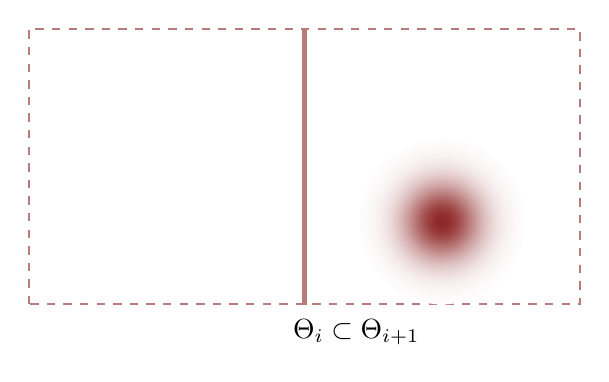
\begin{tikzpicture}[scale=0.35, thick]

  \draw[color=mid, dashed] (-10, -5) rectangle (10, 5);
  
  \fill[color=mid] (-0.1, -5.04) rectangle (0.1, 5.04);

  \node[align=left] at (2.05, -6) { $\Theta_{i} \subset \Theta_{i + 1}$ };

  \foreach \i in {3, 2.98, ..., 0} {
    \pgfmathsetmacro{\prop}{100 * exp(-0.5 * \i * \i)};
    \colorlet{custom}{dark!\prop!white};
    \pgfmathsetmacro{\dy}{\i}
    \fill[color=dark, custom] (5, -2) circle ({1 * \i} and {1 * \i});
  }

\end{tikzpicture}

\end{document}  